\RequirePackage[l2tabu, orthodox]{nag} %Check for obsolete commands
\documentclass[canadien,12pt,oneside,letterpaper]{article}
%
%-----------------------------------------------------
%Loading packages
%
\usepackage[utf8]{inputenc}
\usepackage[T1]{fontenc}
\usepackage[canadien]{babel}
\usepackage{lmodern}
\usepackage{textcomp}
\usepackage{amsmath,amssymb}
\usepackage{siunitx}
\usepackage[svgnames]{xcolor}
\usepackage{hyperref}
\usepackage[all]{hypcap}
\usepackage{graphicx}
\usepackage[oldvoltagedirection,americanvoltages,americancurrents,siunitx]{circuitikz}
\usetikzlibrary{babel}
\usepackage{pgfplots}
\pgfplotsset{compat=1.15}
\usepackage{mathrsfs}
\usetikzlibrary{arrows}
\usepackage{caption}
%\usepackage{subcaption}
\usepackage{subfig}
\usepackage[letterpaper,headheight=15pt]{geometry}
\usepackage{fancyhdr}
\usepackage{setspace}
%
\captionsetup{font=small,labelfont=bf,margin=0.1\textwidth}
\pagestyle{myheadings}
\markboth{PHY-2002/GPH-2006~---~Analyse~fréquentielle}{PHY-2002/GPH-2006~---~Arduino}

\begin{document}

\title{\textbf{Complément}\\Arduino}
\author{Samuel Nadeau \& Claudine Allen}
\date{}
\maketitle

\subsection*{Carte de contrôle et d'acquistion Arduino UNO}
Un survol rapide de la carte Arduino UNO, raccourci à Arduino par la suite, est présenté dans cette section, mais de nombreuses autres ressources se retrouvent facilement sur Internet. Un bon point de départ dans le cadre de ce projet de conception est la liste de \href{https://www.youtube.com/playlist?list=PLV6cmKvnKRs5geApVORPW79U6s3wpa0Ht}{vidéos préparés par l'équipe de Tinkercad}. Ces vidéos initient à l'utilisation d'Arduino via la réalisation de quelques projets de base, alors que le texte qui suit, avec plusieurs liens d'informations complémentaires, expliquera la composition de la carte et la base de son fonctionnement. 

\subsubsection*{Qu'est qu'un Arduino?}
À la base, c'est un circuit imprimé sur une carte (\textit{printed circuit board}, PCB) fabriqués par la \href{https://www.arduino.cc/}{ compagnie Arduino}\footnote{La force de la compagnie Arduino est sa mission de développer de l'électronique totalement en accès libre (\textit{open source}), des diagrammes de circuits à la programmation, et de faciliter son usage par tous.tes les utilisateurs.trices et créateurs.trices indépendamment du niveau d'expérience.} (Figure~\ref{fig:ArduinoUNO}). Le niveau de complexité d'une telle carte (\href{https://content.arduino.cc/assets/UNO-TH_Rev3e_sch.pdf}{diagramme}) change notre mode de travail en passant progressivement de l'électronique à l'informatique, mais le programme est en principe directement téléversé et exécuté sur la carte au lieu de la connecter à un ordinateur pour chaque exécution. Ce type de circuit imprimé est donc optimisé pour le développement de systèmes embarqués.

%horloge 2 fois dans le paragraphe suivant?
Les principaux composants d’un Arduino sont: le \href{https://en.wikipedia.org/wiki/Microcontroller}{microcontrôleur} (\textit{microcontroller unit}, MCU), la \href{https://electronics.stackexchange.com/questions/26484/how-arduino-power-supply-works}{source de tension} (\textit{power supply}) et l’\href{https://en.wikipedia.org/wiki/Clock_signal}{horloge interne} (\textit{clock}) basée sur un oscillateur. Le microcontrôleur comprend tous les éléments nécessaires pour être un ordinateur miniature, soit un microprocesseur (\textit{central processing unit}, CPU) qui contient les portes logiques pour faire les calculs, de la mémoire vive, de la mémoire cache, des dizaines de périphériques et une horloge.

\begin{figure}[h]
    \centering
    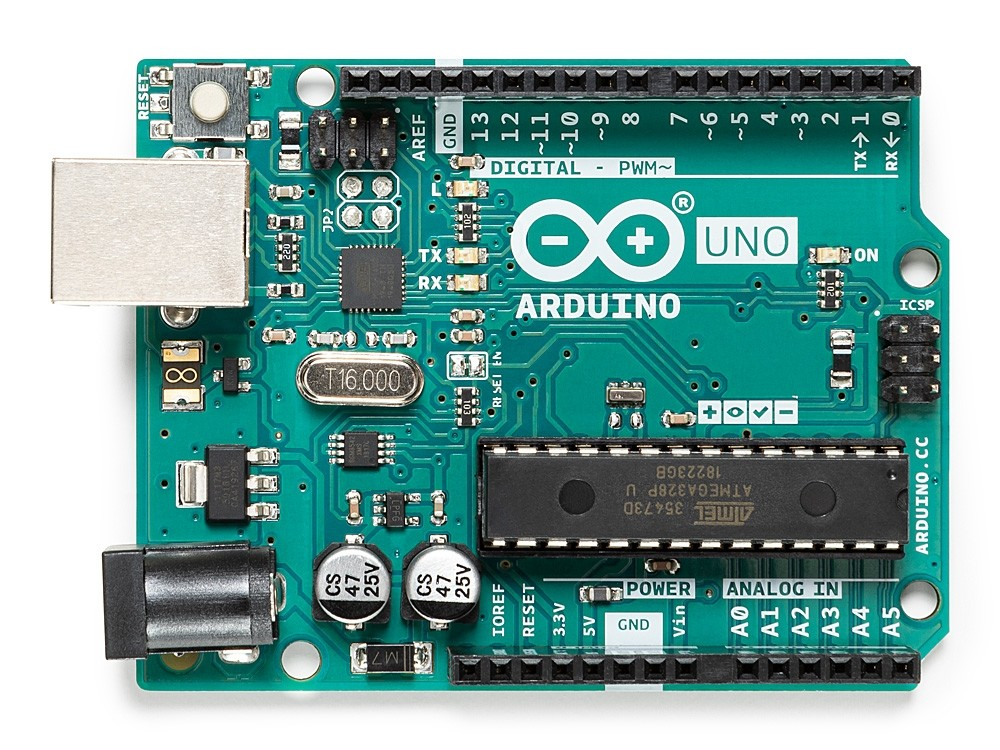
\includegraphics[width=0.3\textwidth]{ArduinoUNO.jpg}
    \caption{La carte Arduino UNO rev3 où la puce principale (longue et noire vers le bas à droite) est le MCU \href{http://ww1.microchip.com/downloads/en/DeviceDoc/Atmel-7810-Automotive-Microcontrollers-ATmega328P_Datasheet.pdf}{ATmega328P} avec des \href{https://www.circuito.io/blog/arduino-uno-pinout/}{ entrées/sorties} situées le long en haut et en bas de la carte alors que l'alimentation et un port USB sont sur la gauche. Photo provenant du \href{https://store.arduino.cc/usa/}{magasin en ligne} de la compagnie Arduino.}
    \label{fig:ArduinoUNO}
\end{figure}

\subsubsection*{Qu'est qu'un Arduino peut faire?}
Cela dépend des périphériques disponibles sur le MCU utilisé, soit ATmega328P de Atmel pour la carte Arduino UNO. Quelques exemples sont de l’acquisition de données, de la synchronisation de signaux, du traitement de données en temps réel, etc. Parmi les périphériques du MCU que l’Arduino utilise, deux (au minimum) seront utiles à la conception du système:
\begin{itemize}
    \item le \href{https://en.wikipedia.org/wiki/Analog-to-digital_converter}{convertisseur analogique-numérique} (\textit{analog-to-digital converter}, ADC) qui permet de lire une tension analogique, par exemple aux bornes d’une photorésistance ou celle qui était fournie par une pomme de terre au début du cours(!),
    \item le générateur de signaux en \href{https://en.wikipedia.org/wiki/Pulse-width_modulation}{modulation de largeur d'impulsions} (\textit{pulse-width modulation}, PWM) qui permet de contrôler certains composants qui ne nécessitent pas un courant élevé, par exemple la base d’un transistor.
\end{itemize}

 Pour utiliser ces fonctionnalités, Arduino a implémenté des fonctions simples à utiliser, soit les fonctions \texttt{AnalogRead}  et \texttt{DigitalWrite/AnalogWrite}. Afin de faire l’acquisition d’un signal avec l’Arduino, les entrées qui sont identifiées \textbf{ADC} ou encore \textbf{A0, A1, A2,} … devront être utilisées. Pour générer un signal, les sorties qui sont identifiées \textbf{PWM} seront utilisées. Arduino, voulant simplifier la tâche, a indiqué que certaines entrées étaient dédiées à des fonctions spécifiques, mais en réalité, c’est le MCU qui décide ce qui se passe sur une entrée et plusieurs fonctions différentes peuvent être utilisées sur une seule et même entrée.
 
\subsubsection*{Comment utiliser un Arduino?}
 En principe, il faut le programmer avec un rapide langage compilé comme le C ou le C++ qui permettra de téléverser le code du programme sur la carte Arduino. Dans notre contexte pédagogique ou toute autre situation se prêtant à laisser l'Arduino branché à un ordinateur complet, vous pouvez alors utiliser des langages interprétés de haut niveau\footnote{Des librairies se développent dans plusieurs langages tels Python (\href{https://github.com/tino/pyFirmata}{pyFirmata}, \href{https://pypi.org/project/pyserial/}{pyserial}, ...) et \href{https://www.mathworks.com/help/supportpkg/arduinoio/examples/getting-started-with-matlab-support-package-for-arduino-hardware.html}{MATLAB} pour communiquer avec une carte Arduino à partir d'un ordinateur ou encore être exécutées directement sur d'autres types de MCU avec \href{https://micropython.org/}{MicroPython} ou \href{https://www.digikey.ca/en/maker/blogs/2018/python-on-hardware}{CircuitPython} par exemple.}. 
 
 %La documentation de base du module se trouve \href{https://pyfirmata.readthedocs.io/en/latest/index.html}{ici}, accompagnée de cette \href{https://pyfirmata.readthedocs.io/en/latest/pyfirmata.html}{liste de classes}. Comme elle est peu détaillée, nous vous recommandons de commencer par consulter ce \textit{\href{https://realpython.com/arduino-python/}{How to}} et n'hésitez pas à partager toute autre ressource que vous trouvez pour faciliter l'usage du module pyFirmata.

La compagnie Arduino offre aussi une \href{https://www.arduino.cc/en/software}{interface de programmation}, aussi installée sur les ordinateurs du laboratoire, qui contient déjà plusieurs fonctions "pré-codées" (\href{https://www.arduino.cc/en/Tutorial/BuiltInExamples}{
didacticiels ici}). Voici quelques conseils si vous souhaitez vous lancer dans cette programmation :
\begin{itemize}
    \item Toutes les variables doivent toutes être déclarées au début, ainsi que leur \href{https://en.wikipedia.org/wiki/C_data_types}{type} avant de les utiliser ailleurs dans le code.
    \item La fonction \texttt{void functionName()~\{\}} signifie seulement que la fonction ne retourne rien, car il faut aussi déclarer ce que la fonction retourne. Si la fonction retourne un entier, il faut plutôt écrire \texttt{int functionName()~\{\}}.
    \item L’intégralité de ce qui se passe lorsque l’Arduino exécute se trouve dans la fonction \texttt{loop()~\{\}}.
    \item Le code dans la fonction \texttt{setup()~\{\}} ne sera exécuté qu’une fois au démarrage de l’Arduino.
    \item Le moniteur série dans Tinkercad permet de faire des actions équivalentes à la commande \texttt{print} rencontrée en Python et bien d'autres langages; cela pourrait simplifier la tâche.
\end{itemize}
 
Si vous préférez utiliser Python pour programmer du code Arduino, on vous suggère fortement d'utiliser la librairie pyFirmata. La documentation de base du module se trouve \href{https://pyfirmata.readthedocs.io/en/latest/index.html}{ici}, accompagnée de cette \href{https://pyfirmata.readthedocs.io/en/latest/pyfirmata.html}{liste de classes}. Comme elle est peu détaillée, nous vous recommandons de commencer par consulter ce \textit{\href{https://realpython.com/arduino-python/}{How to}}. Si vous possédez Python 3.11 et plus, vous ne pourrez cependant pas installer pyFirmata avec un simple \textit{pip install} car la version de pyFirmata qui se trouve sur le \href{https://pypi.org/}{Python Package Index} utilise une fonction qui n'existe plus à partir de Python 3.11. Ce problème de compatibilité a été résolu dans une nouvelle version de pyFirmata, mais celle-ci se trouve seulement sur \href{https://github.com/tino/pyFirmata}{Github}. Pour installer cette version, il vous faudra d'abord installer \href{https://git-scm.com/downloads}{Git} sur votre ordinateur. Ensuite, entrez et exécutez la commande suivante dans un terminal:\\ \textbf{pip install git+https://github.com/tino/pyFirmata.git#egg=pyFirmata}
\newline
Finalement, il reste une dernière étape avant que vous puissiez utiliser pyFirmata. Branchez votre Arduino Uno dans votre ordinateur, puis ouvrez le logiciel Arduino IDE. Assurez-vous que le bon port USB a été sélectionné dans le logiciel (ex: COM7) puis allez dans \textit{fichier} \textrightarrow \textit{exemples} \textrightarrow \textit{Firmata} \textrightarrow \textit{StandardFirmata}. 
\begin{center}
    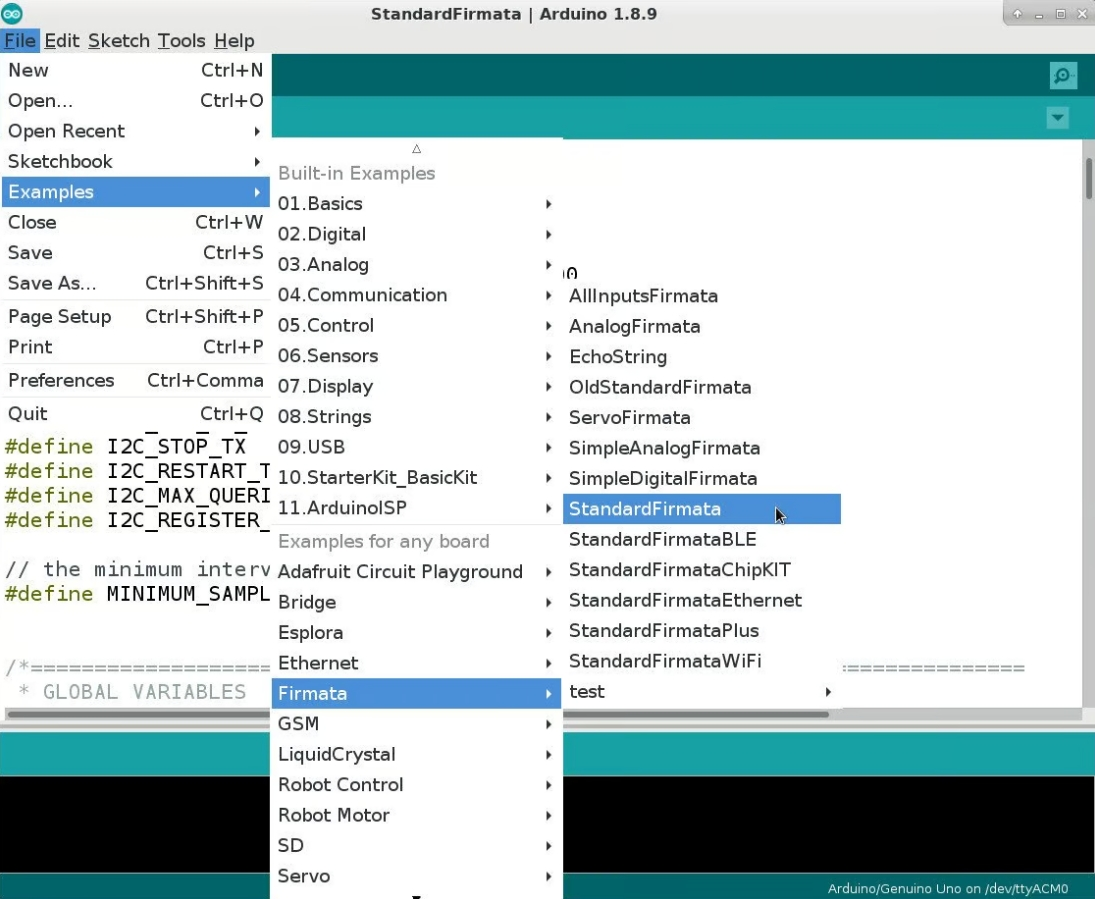
\includegraphics[scale=0.4]{Labos-Complements/Lab07/FirmataSketch.jpeg}
\end{center}
Maintenant, cliquez sur \textit{upload}. Avec ce code de téléversé sur votre Arduino, vous pouvez quitter Arduino IDE et programmer avec pyFirmata sur Python. 
\end{document}